\chapter{Structures de données avancées}

\section{Listes chaînées}
Les \emph{listes chaînées} sont des structures de données composées de \emph{nœuds}, où chaque nœud contient des données et un pointeur vers le nœud suivant. Elles sont utiles pour des opérations d'insertion et de suppression rapides sans nécessiter de réallocation de mémoire.

\begin{figure}[H]
	\centering
	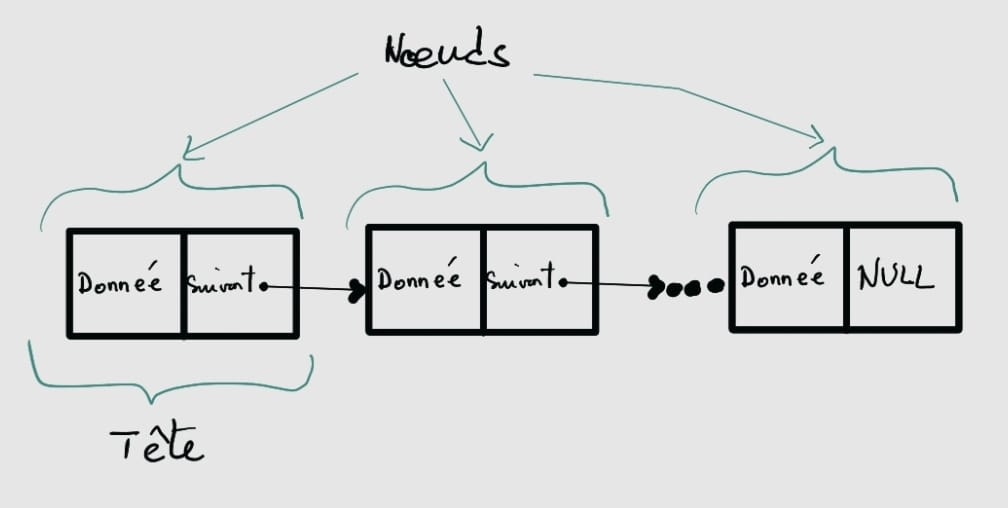
\includegraphics[width=0.8\textwidth]{image/linkedlist}
	\caption{Illustration d'une liste chaînée.}
\end{figure}

\subsection{Création d'une liste chaînée}

Pour créer une liste chaînée, commencez par définir la structure de base du nœud. Chaque nœud contient une donnée (comme un entier) et un pointeur vers le nœud suivant. Initialisez la tête de la liste à \texttt{NULL} pour indiquer qu'elle est vide.

\subsection{Insertion d'un nœud dans la liste chaînée}

Pour insérer un nœud dans une liste chaînée, vous avez deux approches principales:

\begin{itemize}
	\item \textbf{Insérer au début de la liste} : Créez un nouveau nœud, définissez ses données, puis faites pointer ce nœud vers l'ancienne tête de la liste. Mettez ensuite à jour la tête pour qu'elle pointe vers le nouveau nœud.
	
	\item \textbf{Insérer à une position spécifique} : Parcourez la liste jusqu'à la position souhaitée, créez un nouveau nœud, puis ajustez les pointeurs pour insérer le nouveau nœud à la position correcte. Si la position est zéro, insérez au début de la liste.
\end{itemize}

\subsection{Suppression d'un nœud de la liste chaînée}

Pour supprimer un nœud d'une liste chaînée, vous avez deux approches principales:

\begin{itemize}
	\item \textbf{Suppression d'un nœud par clé} : Recherchez un nœud avec une donnée spécifique. Si le nœud à supprimer est la tête de la liste, mettez à jour la tête pour qu'elle pointe vers le nœud suivant. Sinon, ajustez les pointeurs pour déconnecter le nœud du reste de la liste.
	
	\item \textbf{Suppression d'un nœud à une position spécifique} : Parcourez la liste jusqu'à la position spécifiée. Ajustez les pointeurs pour retirer le nœud à cette position. Si la position est hors limites, signalez une erreur.
\end{itemize}

%\subsection{Libération de la liste chaînée}
%
%Après avoir terminé toutes les opérations, il est essentiel de libérer toute la liste chaînée pour éviter des fuites de mémoire. Parcourez la liste, libérez chaque nœud, et assurez-vous que toutes les références à la liste sont annulées.

\subsection{Résumé}

Les listes chaînées offrent une structure flexible pour stocker des données et permettent des opérations d'insertion et de suppression efficaces. L'utilisation de pointeurs est essentielle pour manipuler la structure. Il est également crucial de gérer correctement la mémoire, surtout lors de la suppression de nœuds ou de la libération de la liste entière.

Voici un exemple d'implémentation d'une liste chaînée en C : [Repository containing codes to be pasted here]

\section{Piles}

Les \emph{piles} (ou LIFO, Last In First Out) sont des structures de données où le dernier élément inséré est le premier à être retiré. Les piles sont utiles pour des opérations de retour en arrière, comme dans les navigateurs Web ou les algorithmes de récursion.

\begin{figure}[H]
	\centering
	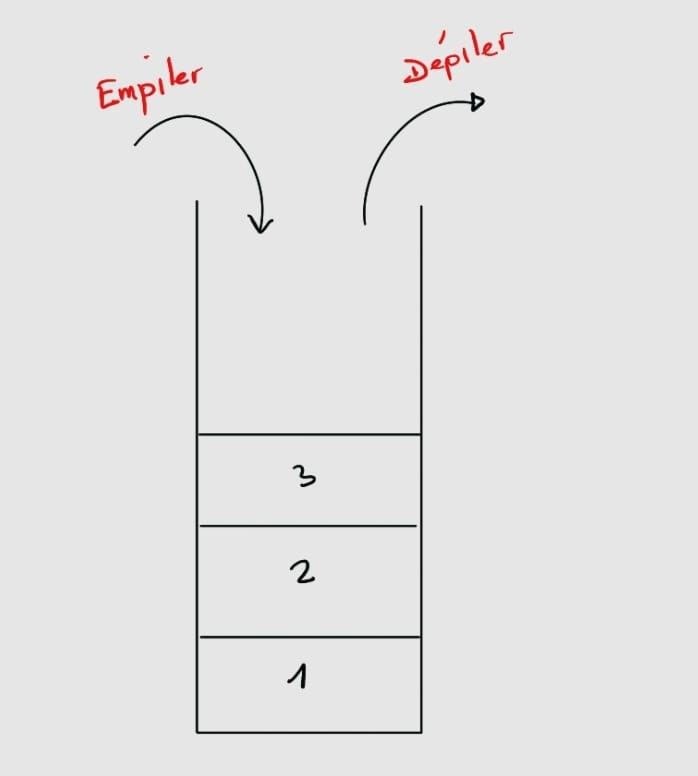
\includegraphics[width=0.5\textwidth]{image/stack} 
	\caption{Illustration d'une pile (LIFO), où le dernier élément ajouté est le premier retiré.}
\end{figure}

\subsection{Construction d'une pile}
Pour construire une pile, vous devez définir une structure qui contient des éléments (comme un tableau ou une liste) et un pointeur ou un indice qui indique le sommet de la pile. Les opérations principales associées aux piles sont l'empilage (ajout d'un élément au sommet) et le dépilage (retrait de l'élément au sommet).

\subsection{Insertion d'un élément dans une pile (empilage)}
L'empilage consiste à ajouter un élément au sommet de la pile. Pour cela, vous devez vérifier si la pile a de la place (si elle n'est pas pleine). Mettez ensuite à jour le sommet pour refléter le nouvel élément. Si vous utilisez un tableau, insérez l'élément à l'indice du sommet. Pour une pile basée sur des listes chaînées, créez un nouveau nœud et ajustez les pointeurs pour insérer le nœud au sommet.

\subsection{Suppression d'un élément dans une pile (dépilage)}
Le dépilage consiste à retirer l'élément au sommet de la pile. Comme pour l'empilage, vérifiez s'il y a des éléments dans la pile (pour éviter de dépiler une pile vide). Si la pile est vide, renvoyez une erreur ou une valeur spéciale pour indiquer qu'il n'y a rien à dépiler. Mettez ensuite à jour le sommet pour refléter le nouvel élément au sommet. Si vous utilisez un tableau, réduisez le sommet d'un indice.

\subsection{Vérification si la pile est vide}
Pour vérifier si la pile est vide, comparez le sommet à -1. Si le sommet est à -1, la pile est vide. Cette vérification est essentielle pour éviter des opérations incorrectes comme le dépilage d'une pile vide, ce qui pourrait causer des erreurs.

\subsection{Utilisations courantes des piles}
Les piles sont utilisées dans de nombreux contextes, tels que les opérations de retour en arrière, les algorithmes de récursion, et les vérifications de syntaxe. Par exemple, les piles sont utiles pour vérifier si des parenthèses sont équilibrées dans une expression mathématique ou de programmation. Elles sont également utilisées dans les navigateurs Web pour gérer l'historique des pages visitées.

\subsection{Résumé}
Les piles offrent une structure simple mais puissante pour gérer des opérations où le dernier entré est le premier à sortir. Elles sont utilisées dans de nombreux domaines informatiques, y compris les algorithmes de récursion et les éditeurs de texte. Comprendre leur fonctionnement et savoir comment les utiliser efficacement est essentiel pour tout développeur.


\section{Files}

Les \emph{files} (ou FIFO, First In First Out) sont des structures de données où le premier élément inséré est le premier à sortir. Contrairement aux piles, où le dernier élément ajouté est le premier à sortir, les files fonctionnent comme des files d'attente dans un magasin, où les premiers arrivés sont les premiers servis.

\begin{figure}[H]
	\centering
	 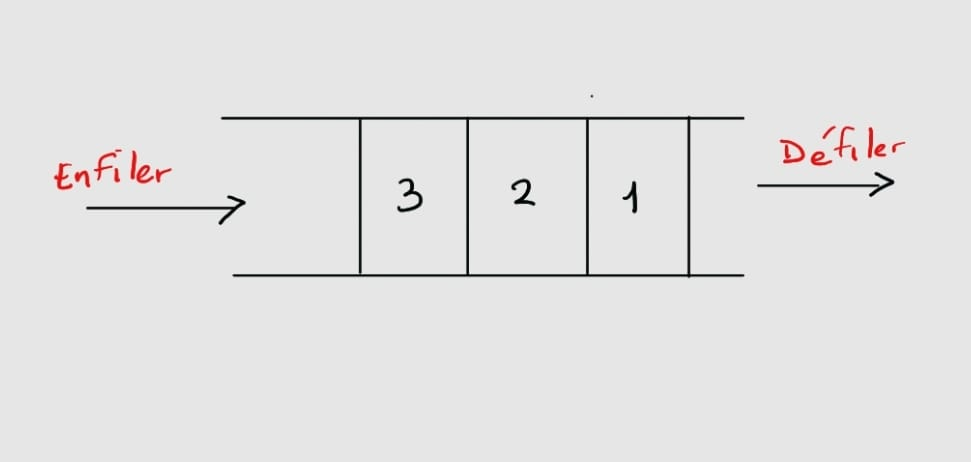
\includegraphics[width=0.8\textwidth]{image/q}  % Exemple d'illustration d'une file
	\caption{Illustration d'une file (FIFO), où le premier élément ajouté est le premier retiré.}
\end{figure}

\subsection{Construction d'une file}
Pour construire une file, définissez une structure qui contient les éléments de la file et des pointeurs vers le début (avant) et la fin (arrière). Cette structure permet des opérations d'enfilage (ajout d'un élément à l'arrière) et de défilage (retrait du premier élément).

\subsection{Insertion d'un élément dans une file (enfilage)}
L'enfilage consiste à ajouter un élément à la fin de la file. Pour cela, assurez-vous qu'il y a de l'espace pour l'élément. Si la file est vide, l'élément ajouté devient à la fois l'avant et l'arrière. Si la file contient déjà des éléments, faites pointer le dernier élément vers le nouveau, puis mettez à jour l'arrière pour indiquer le nouvel élément.

\subsection{Suppression d'un élément dans une file (défilage)}
Le défilage consiste à retirer le premier élément de la file. Avant de le retirer, vérifiez que la file n'est pas vide. Si la file est vide, renvoyez une erreur ou une valeur spéciale. Sinon, mettez à jour l'avant pour qu'il pointe vers le prochain élément, puis libérez la mémoire de l'élément supprimé.

\subsection{Vérification si la file est vide}
Pour vérifier si la file est vide, voyez si l'avant est `NULL`. Si c'est le cas, la file n'a aucun élément, ce qui signifie que vous ne pouvez pas effectuer de défilage. Cette vérification empêche des erreurs liées au défilage d'une file vide.

\subsection{Utilisations courantes des files}
Les files sont largement utilisées dans des applications informatiques où des tâches doivent être effectuées dans un ordre spécifique. Par exemple, les files sont utilisées pour la gestion des tâches, les files d'attente dans les systèmes, et les algorithmes de parcours. Elles sont également utiles pour des structures comme les queues d'impression, les files d'attente dans les réseaux, ou les systèmes d'exploitation qui gèrent des processus.

\subsection{Résumé}
Les files offrent une structure pratique pour des opérations où le premier élément inséré est le premier à sortir. Elles ont de nombreuses applications dans le monde informatique, de la gestion des tâches aux systèmes de files d'attente. Comprendre leur fonctionnement est essentiel pour travailler efficacement avec des structures FIFO.

\section{Arbres binaires}

Les \emph{arbres binaires} sont des structures de données où chaque nœud a au maximum deux enfants. Ils sont souvent utilisés pour des opérations de recherche, de tri, et pour implémenter des algorithmes de parcours comme le pré-ordre, l'en-ordre, et le post-ordre.

\begin{figure}[H]
	\centering
	 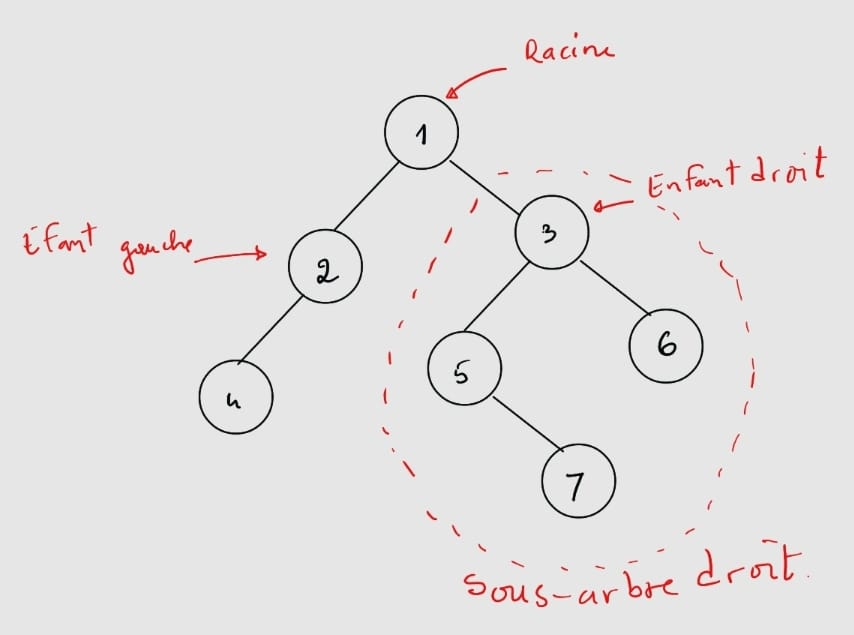
\includegraphics[width=0.8\textwidth]{image/binary_tree}  % Exemple d'illustration d'un arbre binaire
	\caption{Illustration d'un arbre binaire}
\end{figure}

\subsection{Construction d'un arbre binaire}
Pour construire un arbre binaire, définissez une structure de nœud qui contient des données (comme un entier) et des pointeurs vers les enfants gauche et droit. L'arbre binaire commence avec un seul nœud racine, et les autres nœuds sont ajoutés en fonction de leur relation avec le racine.

\subsection{Insertion dans un arbre binaire}
Pour insérer un élément dans un arbre binaire, commencez par la racine. Si le nouvel élément est plus petit que le racine, allez à gauche. S'il est plus grand, allez à droite. Continuez à descendre jusqu'à ce que vous trouviez une position vide. Ajoutez alors un nouveau nœud à cet endroit.

\subsection{Utilisations courantes des arbres binaires}
Les arbres binaires sont largement utilisés dans des algorithmes informatiques. Ils permettent des opérations de recherche rapides car les éléments peuvent être trouvés sans parcourir tout l'arbre. Les arbres binaires peuvent être utilisés pour des opérations comme la recherche binaire, le tri d'arbres, et le parcours de différentes manières (pré-ordre, en-ordre, post-ordre).

\subsection{Algorithmes de parcours des arbres binaires}

Les algorithmes de parcours des arbres binaires permettent d'explorer ou de traverser les arbres de différentes manières. Les méthodes courantes de parcours sont le parcours en-ordre, le parcours pré-ordre, et le parcours post-ordre.

\begin{enumerate}[label=\alph*)]
	\item \textbf{Parcours en-ordre}
	
	Le parcours en-ordre consiste à visiter les nœuds d'un arbre binaire dans un ordre spécifique : d'abord le sous-arbre gauche, puis le nœud actuel, et enfin le sous-arbre droit. Cette méthode est souvent utilisée pour obtenir les éléments dans un ordre trié.
	
	- Fonctionnement : Commencez par le sous-arbre gauche, puis visitez le nœud actuel, et terminez par le sous-arbre droit. Cela donne les éléments de l'arbre dans un ordre croissant.
	
	\item \textbf{Parcours pré-ordre}
	
	Le parcours pré-ordre visite d'abord le nœud actuel, puis les sous-arbres gauche et droit. Il est souvent utilisé pour copier des arbres binaires ou pour créer des représentations pré-ordre.
	
	- Fonctionnement : Visitez le nœud actuel, puis parcourez le sous-arbre gauche, puis le sous-arbre droit. Cela peut être utilisé pour recréer l'arbre ou explorer tous les nœuds.
	
	\item \textbf{Parcours post-ordre}
	
	Le parcours post-ordre commence par les sous-arbres gauche et droit, puis visite le nœud actuel. Cette méthode est souvent utilisée pour supprimer des arbres ou pour des opérations nécessitant une évaluation de bas en haut.
	
	- Fonctionnement : Commencez par le sous-arbre gauche, puis le sous-arbre droit, et enfin visitez le nœud actuel. Ce parcours est utile pour des opérations de suppression ou de nettoyage d'arbre.
	
\end{enumerate}

Les algorithmes de parcours des arbres binaires ont des applications variées. Le parcours en-ordre est idéal pour obtenir des éléments dans un ordre trié, le pré-ordre est utilisé pour copier ou recréer des arbres, et le post-ordre est souvent utilisé pour des opérations de suppression ou de nettoyage. Comprendre ces différentes méthodes de parcours est essentiel pour travailler avec des arbres binaires et résoudre des problèmes complexes d'arborescence.


\subsection{Résumé}
Les arbres binaires sont des structures de données polyvalentes, idéales pour des opérations de recherche et de tri. Ils permettent des algorithmes efficaces pour parcourir des données de manière structurée. Comprendre comment insérer des nœuds et utiliser des arbres binaires est crucial pour travailler avec des structures de données avancées.

\section{Graphes}

Les \emph{graphes} sont des structures de données composées de nœuds (ou sommets) et d'arêtes (les connexions entre les nœuds). Les graphes peuvent être orientés ou non orientés. Dans un graphe orienté, les arêtes ont une direction (comme une flèche). Dans un graphe non orienté, les arêtes n'ont pas de direction particulière. Les graphes sont utilisés pour résoudre des problèmes complexes comme la recherche des plus courts chemins, la détection de cycles, ou le partitionnement.

\begin{figure}[H]
	\centering
	 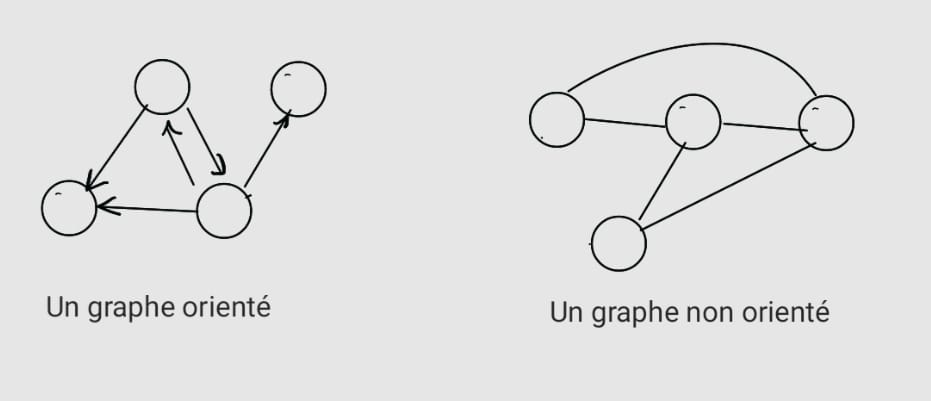
\includegraphics[width=0.8\textwidth]{image/graph}  % Exemple d'illustration d'un graphe
	\caption{Exemples des deux types de graphes}
\end{figure}

\subsection{Construction d'un graphe}
Pour construire un graphe, vous devez définir une structure qui contient une liste de sommets et des arêtes qui les relient. Les graphes peuvent être implémentés de différentes manières, comme avec des listes d'adjacence ou des matrices d'adjacence.

Dans le cas des listes d'adjacence, chaque sommet a une liste de connexions vers d'autres sommets. Les graphes peuvent être orientés (avec des flèches pour indiquer la direction des arêtes) ou non orientés (où les connexions sont bidirectionnelles). Pour construire un graphe, initialisez le nombre de sommets et allouez de la mémoire pour chaque liste d'adjacence.

\subsection{Ajout d'arêtes (liens) dans un graphe}
Pour ajouter des arêtes dans un graphe, vous devez d'abord déterminer les sommets que vous voulez relier. Si le graphe est orienté, assurez-vous de respecter la direction des arêtes. Pour un graphe non orienté, ajoutez des connexions bidirectionnelles. 

Dans le cas des listes d'adjacence, créez un nouveau nœud pour chaque connexion, puis ajoutez-le à la liste du sommet correspondant. Assurez-vous que les arêtes sont correctement ajoutées pour éviter les erreurs de connexion.

\subsection{Utilisations courantes des graphes}
Les graphes sont utilisés dans de nombreux domaines informatiques. Ils permettent de modéliser des relations complexes entre des entités. Par exemple, les graphes peuvent représenter des réseaux de transport, des relations sociales, ou des connexions informatiques. Les graphes sont également utiles pour des algorithmes de parcours comme la recherche en profondeur (DFS) ou la recherche en largeur (BFS).

Les graphes peuvent résoudre des problèmes comme la recherche du plus court chemin, la détection de cycles, et la recherche de composants connexes. Comprendre leur fonctionnement est essentiel pour travailler avec des structures de données avancées.

\subsection{Algorithmes de parcours de graphes}

Les algorithmes de parcours de graphes permettent d'explorer ou de traverser les graphes de différentes manières. Les méthodes courantes de parcours incluent la recherche en profondeur (DFS) et la recherche en largeur (BFS).

\begin{enumerate}[label=\alph*)]
	\item \textbf{Recherche en profondeur (DFS)}
	
	DFS explore le graphe en suivant chaque branche aussi loin que possible avant de revenir en arrière. Elle utilise une pile pour mémoriser les nœuds visités. DFS est souvent utilisée pour détecter des cycles, trouver des composants connexes, ou résoudre des problèmes de recherche de chemins.
	
	- Fonctionnement : DFS commence à partir d'un nœud et explore tous ses voisins. Ensuite, il passe au nœud suivant non visité, poursuivant ainsi la profondeur jusqu'à ce qu'il n'y ait plus de nœuds à visiter. Puis, il revient en arrière pour explorer d'autres chemins.
	
	\item \textbf{Recherche en largeur (BFS)}
	
	BFS explore le graphe couche par couche, en visitant tous les voisins d'un nœud avant de passer au suivant. Elle utilise une file pour mémoriser les nœuds à visiter. BFS est couramment utilisée pour trouver des plus courts chemins dans des graphes non pondérés ou pour des problèmes de recherche de niveaux.
	
	- Fonctionnement : BFS commence par le premier nœud et visite tous ses voisins. Ensuite, il passe aux voisins de ces voisins, touchant tous les nœuds au même niveau avant de passer au niveau suivant.
	
\end{enumerate}

Les algorithmes de parcours de graphes ont des applications variées. DFS est utilisé pour des analyses approfondies, comme la recherche de cycles ou de chemins profonds, tandis que BFS est idéal pour des analyses en surface, comme trouver des connexions courtes ou explorer des niveaux. Ces algorithmes sont essentiels pour résoudre des problèmes complexes de graphes.


\subsection{Résumé}

Les graphes sont des structures de données puissantes qui permettent de modéliser des connexions entre des sommets. Ils sont utilisés dans de nombreux domaines, comme les réseaux informatiques, les systèmes de transport, ou l'analyse sociale. Les graphes peuvent être orientés (où les arêtes ont une direction) ou non orientés (où les connexions sont bidirectionnelles).

Les algorithmes de parcours comme la recherche en profondeur (DFS) et la recherche en largeur (BFS) sont des outils essentiels pour travailler avec des graphes. DFS explore les graphes en profondeur, tandis que BFS explore les graphes en largeur, offrant des applications diverses pour des problèmes complexes.

Les graphes peuvent résoudre des problèmes tels que la recherche des plus courts chemins, la détection de cycles, ou la recherche de composants connexes. Ils permettent également de modéliser des systèmes complexes avec des connexions multiples. La compréhension des graphes, de leurs applications et des algorithmes de parcours est essentielle pour résoudre des problèmes avancés en informatique.

